\documentclass[1p]{elsarticle_modified}
%\bibliographystyle{elsarticle-num}

%\usepackage[colorlinks]{hyperref}
%\usepackage{abbrmath_seonhwa} %\Abb, \Ascr, \Acal ,\Abf, \Afrak
\usepackage{amsfonts}
\usepackage{amssymb}
\usepackage{amsmath}
\usepackage{amsthm}
\usepackage{scalefnt}
\usepackage{amsbsy}
\usepackage{kotex}
\usepackage{caption}
\usepackage{subfig}
\usepackage{color}
\usepackage{graphicx}
\usepackage{xcolor} %% white, black, red, green, blue, cyan, magenta, yellow
\usepackage{float}
\usepackage{setspace}
\usepackage{hyperref}

\usepackage{tikz}
\usetikzlibrary{arrows}

\usepackage{multirow}
\usepackage{array} % fixed length table
\usepackage{hhline}

%%%%%%%%%%%%%%%%%%%%%
\makeatletter
\renewcommand*\env@matrix[1][\arraystretch]{%
	\edef\arraystretch{#1}%
	\hskip -\arraycolsep
	\let\@ifnextchar\new@ifnextchar
	\array{*\c@MaxMatrixCols c}}
\makeatother %https://tex.stackexchange.com/questions/14071/how-can-i-increase-the-line-spacing-in-a-matrix
%%%%%%%%%%%%%%%

\usepackage[normalem]{ulem}

\newcommand{\msout}[1]{\ifmmode\text{\sout{\ensuremath{#1}}}\else\sout{#1}\fi}
%SOURCE: \msout is \stkout macro in https://tex.stackexchange.com/questions/20609/strikeout-in-math-mode

\newcommand{\cancel}[1]{
	\ifmmode
	{\color{red}\msout{#1}}
	\else
	{\color{red}\sout{#1}}
	\fi
}

\newcommand{\add}[1]{
	{\color{blue}\uwave{#1}}
}

\newcommand{\replace}[2]{
	\ifmmode
	{\color{red}\msout{#1}}{\color{blue}\uwave{#2}}
	\else
	{\color{red}\sout{#1}}{\color{blue}\uwave{#2}}
	\fi
}

\newcommand{\Sol}{\mathcal{S}} %segment
\newcommand{\D}{D} %diagram
\newcommand{\A}{\mathcal{A}} %arc


%%%%%%%%%%%%%%%%%%%%%%%%%%%%%5 test

\def\sl{\operatorname{\textup{SL}}(2,\Cbb)}
\def\psl{\operatorname{\textup{PSL}}(2,\Cbb)}
\def\quan{\mkern 1mu \triangleright \mkern 1mu}

\theoremstyle{definition}
\newtheorem{thm}{Theorem}[section]
\newtheorem{prop}[thm]{Proposition}
\newtheorem{lem}[thm]{Lemma}
\newtheorem{ques}[thm]{Question}
\newtheorem{cor}[thm]{Corollary}
\newtheorem{defn}[thm]{Definition}
\newtheorem{exam}[thm]{Example}
\newtheorem{rmk}[thm]{Remark}
\newtheorem{alg}[thm]{Algorithm}

\newcommand{\I}{\sqrt{-1}}
\begin{document}

%\begin{frontmatter}
%
%\title{Boundary parabolic representations of knots up to 8 crossings}
%
%%% Group authors per affiliation:
%\author{Yunhi Cho} 
%\address{Department of Mathematics, University of Seoul, Seoul, Korea}
%\ead{yhcho@uos.ac.kr}
%
%
%\author{Seonhwa Kim} %\fnref{s_kim}}
%\address{Center for Geometry and Physics, Institute for Basic Science, Pohang, 37673, Korea}
%\ead{ryeona17@ibs.re.kr}
%
%\author{Hyuk Kim}
%\address{Department of Mathematical Sciences, Seoul National University, Seoul 08826, Korea}
%\ead{hyukkim@snu.ac.kr}
%
%\author{Seokbeom Yoon}
%\address{Department of Mathematical Sciences, Seoul National University, Seoul, 08826,  Korea}
%\ead{sbyoon15@snu.ac.kr}
%
%\begin{abstract}
%We find all boundary parabolic representation of knots up to 8 crossings.
%
%\end{abstract}
%\begin{keyword}
%    \MSC[2010] 57M25 
%\end{keyword}
%
%\end{frontmatter}

%\linenumbers
%\tableofcontents
%
\newcommand\colored[1]{\textcolor{white}{\rule[-0.35ex]{0.8em}{1.4ex}}\kern-0.8em\color{red} #1}%
%\newcommand\colored[1]{\textcolor{white}{ #1}\kern-2.17ex	\textcolor{white}{ #1}\kern-1.81ex	\textcolor{white}{ #1}\kern-2.15ex\color{red}#1	}

{\Large $\underline{12a_{0704}~(K12a_{0704})}$}

\setlength{\tabcolsep}{10pt}
\renewcommand{\arraystretch}{1.6}
\vspace{1cm}\begin{tabular}{m{100pt}>{\centering\arraybackslash}m{274pt}}
\multirow{5}{120pt}{
	\centering
	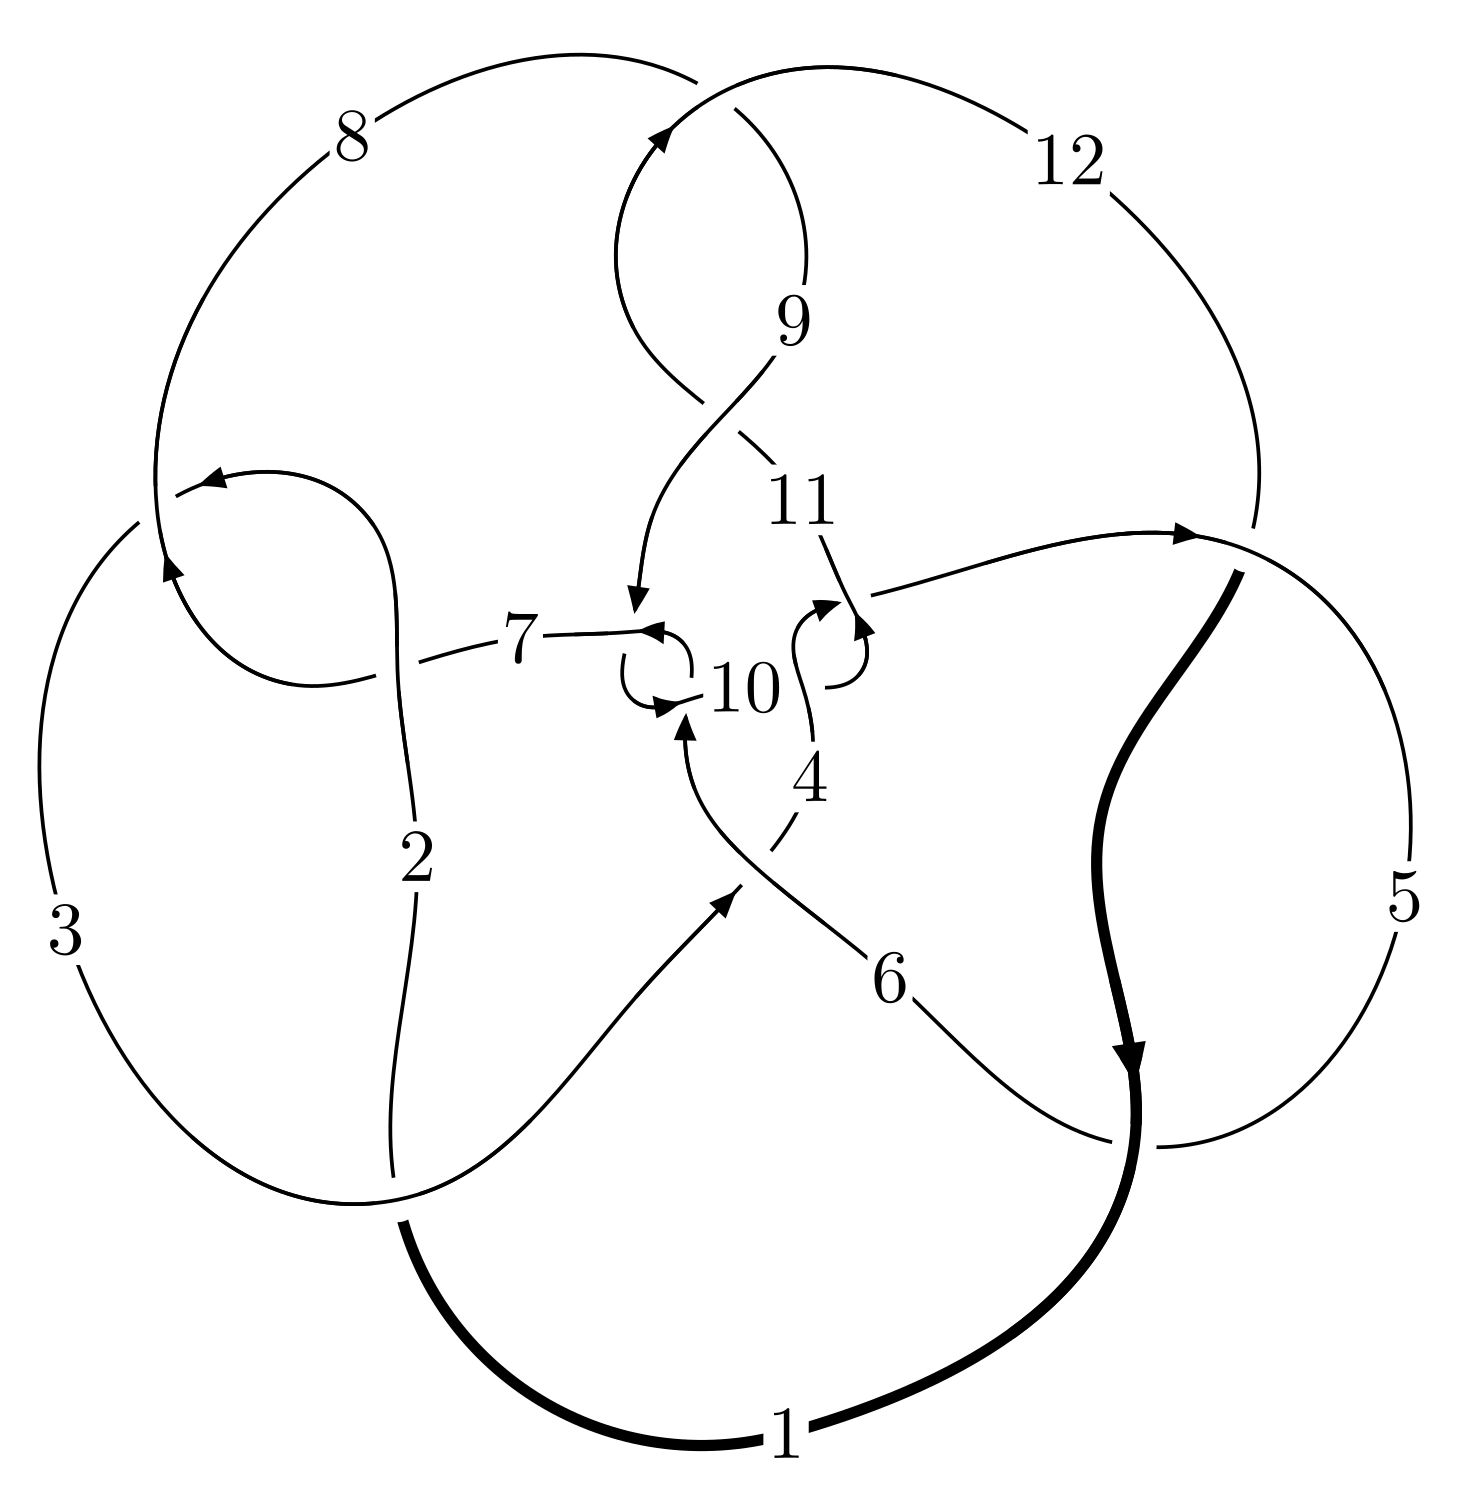
\includegraphics[width=112pt]{../../../GIT/diagram.site/Diagrams/png/1505_12a_0704.png}\\
\ \ \ A knot diagram\footnotemark}&
\allowdisplaybreaks
\textbf{Linearized knot diagam} \\
\cline{2-2}
 &
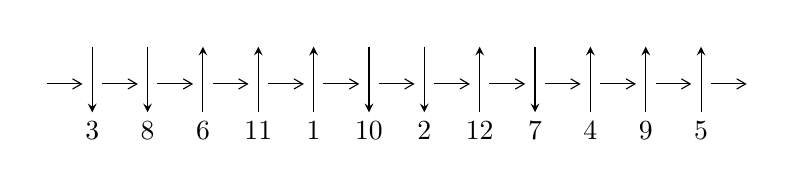
\begin{tikzpicture}[x=20pt, y=17pt]
	% nodes
	\node (C0) at (0, 0) {};
	\node (C1) at (1, 0) {};
	\node (C1U) at (1, +1) {};
	\node (C1D) at (1, -1) {3};

	\node (C2) at (2, 0) {};
	\node (C2U) at (2, +1) {};
	\node (C2D) at (2, -1) {8};

	\node (C3) at (3, 0) {};
	\node (C3U) at (3, +1) {};
	\node (C3D) at (3, -1) {6};

	\node (C4) at (4, 0) {};
	\node (C4U) at (4, +1) {};
	\node (C4D) at (4, -1) {11};

	\node (C5) at (5, 0) {};
	\node (C5U) at (5, +1) {};
	\node (C5D) at (5, -1) {1};

	\node (C6) at (6, 0) {};
	\node (C6U) at (6, +1) {};
	\node (C6D) at (6, -1) {10};

	\node (C7) at (7, 0) {};
	\node (C7U) at (7, +1) {};
	\node (C7D) at (7, -1) {2};

	\node (C8) at (8, 0) {};
	\node (C8U) at (8, +1) {};
	\node (C8D) at (8, -1) {12};

	\node (C9) at (9, 0) {};
	\node (C9U) at (9, +1) {};
	\node (C9D) at (9, -1) {7};

	\node (C10) at (10, 0) {};
	\node (C10U) at (10, +1) {};
	\node (C10D) at (10, -1) {4};

	\node (C11) at (11, 0) {};
	\node (C11U) at (11, +1) {};
	\node (C11D) at (11, -1) {9};

	\node (C12) at (12, 0) {};
	\node (C12U) at (12, +1) {};
	\node (C12D) at (12, -1) {5};
	\node (C13) at (13, 0) {};

	% arrows
	\draw[->,>={angle 60}]
	(C0) edge (C1) (C1) edge (C2) (C2) edge (C3) (C3) edge (C4) (C4) edge (C5) (C5) edge (C6) (C6) edge (C7) (C7) edge (C8) (C8) edge (C9) (C9) edge (C10) (C10) edge (C11) (C11) edge (C12) (C12) edge (C13) ;	\draw[->,>=stealth]
	(C1U) edge (C1D) (C2U) edge (C2D) (C3D) edge (C3U) (C4D) edge (C4U) (C5D) edge (C5U) (C6U) edge (C6D) (C7U) edge (C7D) (C8D) edge (C8U) (C9U) edge (C9D) (C10D) edge (C10U) (C11D) edge (C11U) (C12D) edge (C12U) ;
	\end{tikzpicture} \\
\hhline{~~} \\& 
\textbf{Solving Sequence} \\ \cline{2-2} 
 &
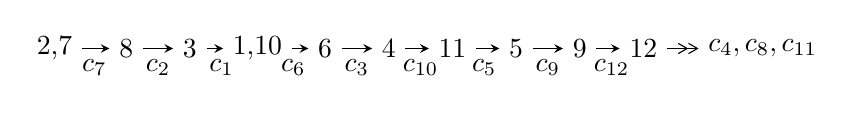
\begin{tikzpicture}[x=23pt, y=7pt]
	% node
	\node (A0) at (-1/8, 0) {2,7};
	\node (A1) at (1, 0) {8};
	\node (A2) at (2, 0) {3};
	\node (A3) at (49/16, 0) {1,10};
	\node (A4) at (33/8, 0) {6};
	\node (A5) at (41/8, 0) {4};
	\node (A6) at (49/8, 0) {11};
	\node (A7) at (57/8, 0) {5};
	\node (A8) at (65/8, 0) {9};
	\node (A9) at (73/8, 0) {12};
	\node (C1) at (1/2, -1) {$c_{7}$};
	\node (C2) at (3/2, -1) {$c_{2}$};
	\node (C3) at (5/2, -1) {$c_{1}$};
	\node (C4) at (29/8, -1) {$c_{6}$};
	\node (C5) at (37/8, -1) {$c_{3}$};
	\node (C6) at (45/8, -1) {$c_{10}$};
	\node (C7) at (53/8, -1) {$c_{5}$};
	\node (C8) at (61/8, -1) {$c_{9}$};
	\node (C9) at (69/8, -1) {$c_{12}$};
	\node (A10) at (11, 0) {$c_{4},c_{8},c_{11}$};

	% edge
	\draw[->,>=stealth]	
	(A0) edge (A1) (A1) edge (A2) (A2) edge (A3) (A3) edge (A4) (A4) edge (A5) (A5) edge (A6) (A6) edge (A7) (A7) edge (A8) (A8) edge (A9) ;
	\draw[->>,>={angle 60}]	
	(A9) edge (A10);
\end{tikzpicture} \\ 

\end{tabular} \\

\footnotetext{
The image of knot diagram is generated by the software ``\textbf{Draw programme}" developed by Andrew Bartholomew(\url{http://www.layer8.co.uk/maths/draw/index.htm\#Running-draw}), where we modified some parts for our purpose(\url{https://github.com/CATsTAILs/LinksPainter}).
}\phantom \\ \newline 
\centering \textbf{Ideals for irreducible components\footnotemark of $X_{\text{par}}$} 
 
\begin{align*}
I^u_{1}&=\langle 
-7.60148\times10^{463} u^{146}+1.63393\times10^{463} u^{145}+\cdots+6.38257\times10^{464} b-5.26299\times10^{466},\\
\phantom{I^u_{1}}&\phantom{= \langle  }1.03268\times10^{467} u^{146}-1.43461\times10^{466} u^{145}+\cdots+3.36361\times10^{467} a+5.88493\times10^{469},\\
\phantom{I^u_{1}}&\phantom{= \langle  }u^{147}- u^{146}+\cdots+1273 u-527\rangle \\
I^u_{2}&=\langle 
5521967436 u^{45}+25712795502 u^{44}+\cdots+1058458619 b-22055868259,\\
\phantom{I^u_{2}}&\phantom{= \langle  }64806150566 u^{45}+33655961613 u^{44}+\cdots+1058458619 a-25765949811,\\
\phantom{I^u_{2}}&\phantom{= \langle  }u^{46}-14 u^{44}+\cdots+2 u+1\rangle \\
\\
\end{align*}
\raggedright * 2 irreducible components of $\dim_{\mathbb{C}}=0$, with total 193 representations.\\
\footnotetext{All coefficients of polynomials are rational numbers. But the coefficients are sometimes approximated in decimal forms when there is not enough margin.}
\newpage
\renewcommand{\arraystretch}{1}
\centering \section*{I. $I^u_{1}= \langle -7.60\times10^{463} u^{146}+1.63\times10^{463} u^{145}+\cdots+6.38\times10^{464} b-5.26\times10^{466},\;1.03\times10^{467} u^{146}-1.43\times10^{466} u^{145}+\cdots+3.36\times10^{467} a+5.88\times10^{469},\;u^{147}- u^{146}+\cdots+1273 u-527 \rangle$}
\flushleft \textbf{(i) Arc colorings}\\
\begin{tabular}{m{7pt} m{180pt} m{7pt} m{180pt} }
\flushright $a_{2}=$&$\begin{pmatrix}0\\u\end{pmatrix}$ \\
\flushright $a_{7}=$&$\begin{pmatrix}1\\0\end{pmatrix}$ \\
\flushright $a_{8}=$&$\begin{pmatrix}1\\u^2\end{pmatrix}$ \\
\flushright $a_{3}=$&$\begin{pmatrix}- u\\- u^3+u\end{pmatrix}$ \\
\flushright $a_{1}=$&$\begin{pmatrix}u^3\\u^5- u^3+u\end{pmatrix}$ \\
\flushright $a_{10}=$&$\begin{pmatrix}-0.307015 u^{146}+0.0426507 u^{145}+\cdots+264.395 u-174.959\\0.119098 u^{146}-0.0255999 u^{145}+\cdots-98.5592 u+82.4588\end{pmatrix}$ \\
\flushright $a_{6}=$&$\begin{pmatrix}0.0335880 u^{146}-0.0499830 u^{145}+\cdots-65.0765 u+47.3200\\0.0868913 u^{146}-0.0208113 u^{145}+\cdots-62.4171 u+61.5742\end{pmatrix}$ \\
\flushright $a_{4}=$&$\begin{pmatrix}-0.191808 u^{146}+0.0571137 u^{145}+\cdots+183.167 u-118.328\\0.0720548 u^{146}-0.0359632 u^{145}+\cdots-62.4195 u+71.3182\end{pmatrix}$ \\
\flushright $a_{11}=$&$\begin{pmatrix}-0.374298 u^{146}+0.0923870 u^{145}+\cdots+300.030 u-232.677\\0.148247 u^{146}-0.0335708 u^{145}+\cdots-121.790 u+85.2752\end{pmatrix}$ \\
\flushright $a_{5}=$&$\begin{pmatrix}0.00283914 u^{146}-0.0381795 u^{145}+\cdots-34.0622 u+25.6472\\0.0728317 u^{146}-0.0237253 u^{145}+\cdots-60.1539 u+57.8352\end{pmatrix}$ \\
\flushright $a_{9}=$&$\begin{pmatrix}-0.187918 u^{146}+0.0170508 u^{145}+\cdots+165.835 u-92.4997\\0.119098 u^{146}-0.0255999 u^{145}+\cdots-98.5592 u+82.4588\end{pmatrix}$ \\
\flushright $a_{12}=$&$\begin{pmatrix}-0.0766419 u^{146}+0.00138737 u^{145}+\cdots+32.4750 u-28.5523\\0.0407402 u^{146}+0.00299541 u^{145}+\cdots-25.7432 u+17.3077\end{pmatrix}$\\&\end{tabular}
\flushleft \textbf{(ii) Obstruction class $= -1$}\\~\\
\flushleft \textbf{(iii) Cusp Shapes $= -1.17353 u^{146}+0.321754 u^{145}+\cdots+866.505 u-865.889$}\\~\\
\newpage\renewcommand{\arraystretch}{1}
\flushleft \textbf{(iv) u-Polynomials at the component}\newline \\
\begin{tabular}{m{50pt}|m{274pt}}
Crossings & \hspace{64pt}u-Polynomials at each crossing \\
\hline $$\begin{aligned}c_{1}\end{aligned}$$&$\begin{aligned}
&u^{147}+65 u^{146}+\cdots+6797777 u+277729
\end{aligned}$\\
\hline $$\begin{aligned}c_{2},c_{7}\end{aligned}$$&$\begin{aligned}
&u^{147}- u^{146}+\cdots+1273 u-527
\end{aligned}$\\
\hline $$\begin{aligned}c_{3}\end{aligned}$$&$\begin{aligned}
&u^{147}+5 u^{146}+\cdots-487893741 u+95956559
\end{aligned}$\\
\hline $$\begin{aligned}c_{4},c_{10}\end{aligned}$$&$\begin{aligned}
&u^{147}+u^{146}+\cdots-434404 u-73112
\end{aligned}$\\
\hline $$\begin{aligned}c_{5},c_{12}\end{aligned}$$&$\begin{aligned}
&u^{147}-3 u^{146}+\cdots-1819273 u-573163
\end{aligned}$\\
\hline $$\begin{aligned}c_{6},c_{9}\end{aligned}$$&$\begin{aligned}
&u^{147}-2 u^{146}+\cdots-976586 u+350333
\end{aligned}$\\
\hline $$\begin{aligned}c_{8},c_{11}\end{aligned}$$&$\begin{aligned}
&u^{147}+6 u^{146}+\cdots-10 u-1
\end{aligned}$\\
\hline
\end{tabular}\\~\\
\newpage\renewcommand{\arraystretch}{1}
\flushleft \textbf{(v) Riley Polynomials at the component}\newline \\
\begin{tabular}{m{50pt}|m{274pt}}
Crossings & \hspace{64pt}Riley Polynomials at each crossing \\
\hline $$\begin{aligned}c_{1}\end{aligned}$$&$\begin{aligned}
&y^{147}+59 y^{146}+\cdots-2005730840055 y-77133397441
\end{aligned}$\\
\hline $$\begin{aligned}c_{2},c_{7}\end{aligned}$$&$\begin{aligned}
&y^{147}-65 y^{146}+\cdots+6797777 y-277729
\end{aligned}$\\
\hline $$\begin{aligned}c_{3}\end{aligned}$$&$\begin{aligned}
&y^{147}-75 y^{146}+\cdots+857754722402922901 y-9207661215120481
\end{aligned}$\\
\hline $$\begin{aligned}c_{4},c_{10}\end{aligned}$$&$\begin{aligned}
&y^{147}-109 y^{146}+\cdots-76435879920 y-5345364544
\end{aligned}$\\
\hline $$\begin{aligned}c_{5},c_{12}\end{aligned}$$&$\begin{aligned}
&y^{147}-103 y^{146}+\cdots+11878213249293 y-328515824569
\end{aligned}$\\
\hline $$\begin{aligned}c_{6},c_{9}\end{aligned}$$&$\begin{aligned}
&y^{147}+102 y^{146}+\cdots-10016924047636 y-122733210889
\end{aligned}$\\
\hline $$\begin{aligned}c_{8},c_{11}\end{aligned}$$&$\begin{aligned}
&y^{147}+74 y^{146}+\cdots+496 y-1
\end{aligned}$\\
\hline
\end{tabular}\\~\\
\newpage\flushleft \textbf{(vi) Complex Volumes and Cusp Shapes}
$$\begin{array}{c|c|c}  
\text{Solutions to }I^u_{1}& \I (\text{vol} + \sqrt{-1}CS) & \text{Cusp shape}\\
 \hline 
\begin{aligned}
u &= \phantom{-}0.778426 + 0.640882 I \\
a &= \phantom{-}0.472111 + 1.067180 I \\
b &= -1.54249 - 0.15023 I\end{aligned}
 & \phantom{-}0.127554 - 0.538258 I & \phantom{-0.000000 } 0 \\ \hline\begin{aligned}
u &= \phantom{-}0.778426 - 0.640882 I \\
a &= \phantom{-}0.472111 - 1.067180 I \\
b &= -1.54249 + 0.15023 I\end{aligned}
 & \phantom{-}0.127554 + 0.538258 I & \phantom{-0.000000 } 0 \\ \hline\begin{aligned}
u &= \phantom{-}0.920265 + 0.340469 I \\
a &= -0.65259 - 1.57181 I \\
b &= \phantom{-}0.429836 - 0.752106 I\end{aligned}
 & -0.036251 + 0.731182 I & \phantom{-0.000000 } 0 \\ \hline\begin{aligned}
u &= \phantom{-}0.920265 - 0.340469 I \\
a &= -0.65259 + 1.57181 I \\
b &= \phantom{-}0.429836 + 0.752106 I\end{aligned}
 & -0.036251 - 0.731182 I & \phantom{-0.000000 } 0 \\ \hline\begin{aligned}
u &= \phantom{-}0.356734 + 0.957481 I \\
a &= -0.12746 - 1.71970 I \\
b &= \phantom{-}0.152177 + 1.223830 I\end{aligned}
 & \phantom{-}11.10520 - 1.67996 I & \phantom{-0.000000 } 0 \\ \hline\begin{aligned}
u &= \phantom{-}0.356734 - 0.957481 I \\
a &= -0.12746 + 1.71970 I \\
b &= \phantom{-}0.152177 - 1.223830 I\end{aligned}
 & \phantom{-}11.10520 + 1.67996 I & \phantom{-0.000000 } 0 \\ \hline\begin{aligned}
u &= \phantom{-}0.541223 + 0.872467 I \\
a &= -0.10006 + 1.86950 I \\
b &= \phantom{-}0.431756 - 1.343840 I\end{aligned}
 & \phantom{-}12.19500 + 5.90750 I & \phantom{-0.000000 } 0 \\ \hline\begin{aligned}
u &= \phantom{-}0.541223 - 0.872467 I \\
a &= -0.10006 - 1.86950 I \\
b &= \phantom{-}0.431756 + 1.343840 I\end{aligned}
 & \phantom{-}12.19500 - 5.90750 I & \phantom{-0.000000 } 0 \\ \hline\begin{aligned}
u &= \phantom{-}0.511898 + 0.819681 I \\
a &= -0.082419 + 0.534274 I \\
b &= -0.599851 - 0.097815 I\end{aligned}
 & \phantom{-}1.60243 + 2.51217 I & \phantom{-0.000000 } 0 \\ \hline\begin{aligned}
u &= \phantom{-}0.511898 - 0.819681 I \\
a &= -0.082419 - 0.534274 I \\
b &= -0.599851 + 0.097815 I\end{aligned}
 & \phantom{-}1.60243 - 2.51217 I & \phantom{-0.000000 } 0\\
 \hline 
 \end{array}$$\newpage$$\begin{array}{c|c|c}  
\text{Solutions to }I^u_{1}& \I (\text{vol} + \sqrt{-1}CS) & \text{Cusp shape}\\
 \hline 
\begin{aligned}
u &= \phantom{-}0.785232 + 0.556584 I \\
a &= \phantom{-}0.122117 - 0.805763 I \\
b &= \phantom{-}0.631868 - 0.663164 I\end{aligned}
 & \phantom{-}1.012040 - 0.694926 I & \phantom{-0.000000 } 0 \\ \hline\begin{aligned}
u &= \phantom{-}0.785232 - 0.556584 I \\
a &= \phantom{-}0.122117 + 0.805763 I \\
b &= \phantom{-}0.631868 + 0.663164 I\end{aligned}
 & \phantom{-}1.012040 + 0.694926 I & \phantom{-0.000000 } 0 \\ \hline\begin{aligned}
u &= \phantom{-}0.828523 + 0.636779 I \\
a &= \phantom{-}1.24927 - 2.04135 I \\
b &= \phantom{-}0.79896 + 1.30051 I\end{aligned}
 & \phantom{-}9.83164 - 4.55996 I & \phantom{-0.000000 } 0 \\ \hline\begin{aligned}
u &= \phantom{-}0.828523 - 0.636779 I \\
a &= \phantom{-}1.24927 + 2.04135 I \\
b &= \phantom{-}0.79896 - 1.30051 I\end{aligned}
 & \phantom{-}9.83164 + 4.55996 I & \phantom{-0.000000 } 0 \\ \hline\begin{aligned}
u &= -0.841628 + 0.630253 I \\
a &= \phantom{-}0.953830 - 0.159269 I \\
b &= \phantom{-}0.471205 + 0.705323 I\end{aligned}
 & \phantom{-}1.81516 + 6.04930 I & \phantom{-0.000000 } 0 \\ \hline\begin{aligned}
u &= -0.841628 - 0.630253 I \\
a &= \phantom{-}0.953830 + 0.159269 I \\
b &= \phantom{-}0.471205 - 0.705323 I\end{aligned}
 & \phantom{-}1.81516 - 6.04930 I & \phantom{-0.000000 } 0 \\ \hline\begin{aligned}
u &= -0.573028 + 0.745920 I \\
a &= \phantom{-}0.58729 + 1.74112 I \\
b &= -0.54507 - 1.50557 I\end{aligned}
 & \phantom{-}5.15512 - 6.76066 I & \phantom{-0.000000 } 0 \\ \hline\begin{aligned}
u &= -0.573028 - 0.745920 I \\
a &= \phantom{-}0.58729 - 1.74112 I \\
b &= -0.54507 + 1.50557 I\end{aligned}
 & \phantom{-}5.15512 + 6.76066 I & \phantom{-0.000000 } 0 \\ \hline\begin{aligned}
u &= -0.774357 + 0.519727 I \\
a &= \phantom{-}1.51025 + 3.19257 I \\
b &= \phantom{-}0.273043 - 1.036390 I\end{aligned}
 & \phantom{-}0.83895 + 2.21626 I & \phantom{-0.000000 } 0 \\ \hline\begin{aligned}
u &= -0.774357 - 0.519727 I \\
a &= \phantom{-}1.51025 - 3.19257 I \\
b &= \phantom{-}0.273043 + 1.036390 I\end{aligned}
 & \phantom{-}0.83895 - 2.21626 I & \phantom{-0.000000 } 0\\
 \hline 
 \end{array}$$\newpage$$\begin{array}{c|c|c}  
\text{Solutions to }I^u_{1}& \I (\text{vol} + \sqrt{-1}CS) & \text{Cusp shape}\\
 \hline 
\begin{aligned}
u &= -0.736512 + 0.570399 I \\
a &= -0.352151 + 0.728005 I \\
b &= -0.619511 - 0.998464 I\end{aligned}
 & \phantom{-}2.20503 - 1.16067 I & \phantom{-0.000000 } 0 \\ \hline\begin{aligned}
u &= -0.736512 - 0.570399 I \\
a &= -0.352151 - 0.728005 I \\
b &= -0.619511 + 0.998464 I\end{aligned}
 & \phantom{-}2.20503 + 1.16067 I & \phantom{-0.000000 } 0 \\ \hline\begin{aligned}
u &= -0.634955 + 0.864567 I \\
a &= \phantom{-}0.410494 - 0.446785 I \\
b &= -1.326540 - 0.139935 I\end{aligned}
 & \phantom{-}4.95565 - 6.44680 I & \phantom{-0.000000 } 0 \\ \hline\begin{aligned}
u &= -0.634955 - 0.864567 I \\
a &= \phantom{-}0.410494 + 0.446785 I \\
b &= -1.326540 + 0.139935 I\end{aligned}
 & \phantom{-}4.95565 + 6.44680 I & \phantom{-0.000000 } 0 \\ \hline\begin{aligned}
u &= \phantom{-}1.07508\phantom{ +0.000000I} \\
a &= -0.912775\phantom{ +0.000000I} \\
b &= -0.770574\phantom{ +0.000000I}\end{aligned}
 & \phantom{-}2.41716\phantom{ +0.000000I} & \phantom{-0.000000 } 0 \\ \hline\begin{aligned}
u &= -0.761395 + 0.759469 I \\
a &= -0.92997 - 1.67614 I \\
b &= \phantom{-}0.25336 + 1.46998 I\end{aligned}
 & \phantom{-}7.01462 - 1.27991 I & \phantom{-0.000000 } 0 \\ \hline\begin{aligned}
u &= -0.761395 - 0.759469 I \\
a &= -0.92997 + 1.67614 I \\
b &= \phantom{-}0.25336 - 1.46998 I\end{aligned}
 & \phantom{-}7.01462 + 1.27991 I & \phantom{-0.000000 } 0 \\ \hline\begin{aligned}
u &= \phantom{-}0.842370 + 0.670276 I \\
a &= -0.90569 + 1.87573 I \\
b &= -0.098364 - 1.236020 I\end{aligned}
 & \phantom{-}3.16395 - 2.59138 I & \phantom{-0.000000 } 0 \\ \hline\begin{aligned}
u &= \phantom{-}0.842370 - 0.670276 I \\
a &= -0.90569 - 1.87573 I \\
b &= -0.098364 + 1.236020 I\end{aligned}
 & \phantom{-}3.16395 + 2.59138 I & \phantom{-0.000000 } 0 \\ \hline\begin{aligned}
u &= -0.864504 + 0.649729 I \\
a &= -1.114200 - 0.142895 I \\
b &= -0.622297 + 0.429015 I\end{aligned}
 & \phantom{-}1.73673 - 1.05522 I & \phantom{-0.000000 } 0\\
 \hline 
 \end{array}$$\newpage$$\begin{array}{c|c|c}  
\text{Solutions to }I^u_{1}& \I (\text{vol} + \sqrt{-1}CS) & \text{Cusp shape}\\
 \hline 
\begin{aligned}
u &= -0.864504 - 0.649729 I \\
a &= -1.114200 + 0.142895 I \\
b &= -0.622297 - 0.429015 I\end{aligned}
 & \phantom{-}1.73673 + 1.05522 I & \phantom{-0.000000 } 0 \\ \hline\begin{aligned}
u &= \phantom{-}0.922929 + 0.582561 I \\
a &= -0.291109 + 0.376979 I \\
b &= -0.751318 - 0.383558 I\end{aligned}
 & \phantom{-}0.54199 - 3.86844 I & \phantom{-0.000000 } 0 \\ \hline\begin{aligned}
u &= \phantom{-}0.922929 - 0.582561 I \\
a &= -0.291109 - 0.376979 I \\
b &= -0.751318 + 0.383558 I\end{aligned}
 & \phantom{-}0.54199 + 3.86844 I & \phantom{-0.000000 } 0 \\ \hline\begin{aligned}
u &= \phantom{-}0.830577 + 0.365011 I \\
a &= \phantom{-}0.012926 + 0.482356 I \\
b &= -0.562755 - 0.628357 I\end{aligned}
 & \phantom{-}0.01525 - 3.33985 I & \phantom{-0.000000 } 0 \\ \hline\begin{aligned}
u &= \phantom{-}0.830577 - 0.365011 I \\
a &= \phantom{-}0.012926 - 0.482356 I \\
b &= -0.562755 + 0.628357 I\end{aligned}
 & \phantom{-}0.01525 + 3.33985 I & \phantom{-0.000000 } 0 \\ \hline\begin{aligned}
u &= -0.955020 + 0.544768 I \\
a &= \phantom{-}1.49599 + 2.23878 I \\
b &= -0.054886 - 1.040640 I\end{aligned}
 & \phantom{-}0.21240 + 2.08501 I & \phantom{-0.000000 } 0 \\ \hline\begin{aligned}
u &= -0.955020 - 0.544768 I \\
a &= \phantom{-}1.49599 - 2.23878 I \\
b &= -0.054886 + 1.040640 I\end{aligned}
 & \phantom{-}0.21240 - 2.08501 I & \phantom{-0.000000 } 0 \\ \hline\begin{aligned}
u &= \phantom{-}0.882596 + 0.657710 I \\
a &= \phantom{-}0.894460 - 1.041250 I \\
b &= -0.65403 + 1.39196 I\end{aligned}
 & \phantom{-}9.65804 - 0.48101 I & \phantom{-0.000000 } 0 \\ \hline\begin{aligned}
u &= \phantom{-}0.882596 - 0.657710 I \\
a &= \phantom{-}0.894460 + 1.041250 I \\
b &= -0.65403 - 1.39196 I\end{aligned}
 & \phantom{-}9.65804 + 0.48101 I & \phantom{-0.000000 } 0 \\ \hline\begin{aligned}
u &= \phantom{-}1.096650 + 0.094685 I \\
a &= \phantom{-}1.28110 + 0.88681 I \\
b &= \phantom{-}0.661377 - 0.018405 I\end{aligned}
 & -1.73830 - 5.76419 I & \phantom{-0.000000 } 0\\
 \hline 
 \end{array}$$\newpage$$\begin{array}{c|c|c}  
\text{Solutions to }I^u_{1}& \I (\text{vol} + \sqrt{-1}CS) & \text{Cusp shape}\\
 \hline 
\begin{aligned}
u &= \phantom{-}1.096650 - 0.094685 I \\
a &= \phantom{-}1.28110 - 0.88681 I \\
b &= \phantom{-}0.661377 + 0.018405 I\end{aligned}
 & -1.73830 + 5.76419 I & \phantom{-0.000000 } 0 \\ \hline\begin{aligned}
u &= -0.869444 + 0.202717 I \\
a &= \phantom{-}1.28699 + 1.50201 I \\
b &= \phantom{-}0.980292 - 0.454294 I\end{aligned}
 & -2.87525 - 0.00985 I & \phantom{-0.000000 } 0 \\ \hline\begin{aligned}
u &= -0.869444 - 0.202717 I \\
a &= \phantom{-}1.28699 - 1.50201 I \\
b &= \phantom{-}0.980292 + 0.454294 I\end{aligned}
 & -2.87525 + 0.00985 I & \phantom{-0.000000 } 0 \\ \hline\begin{aligned}
u &= -0.508186 + 0.729992 I \\
a &= -0.618628 + 0.050688 I \\
b &= \phantom{-}0.795914 + 0.101504 I\end{aligned}
 & \phantom{-}7.73827 - 1.29712 I & \phantom{-0.000000 } 0 \\ \hline\begin{aligned}
u &= -0.508186 - 0.729992 I \\
a &= -0.618628 - 0.050688 I \\
b &= \phantom{-}0.795914 - 0.101504 I\end{aligned}
 & \phantom{-}7.73827 + 1.29712 I & \phantom{-0.000000 } 0 \\ \hline\begin{aligned}
u &= -0.951941 + 0.576556 I \\
a &= \phantom{-}1.73167 + 0.74324 I \\
b &= \phantom{-}0.672415 - 0.868583 I\end{aligned}
 & \phantom{-}1.51005 + 5.75445 I & \phantom{-0.000000 } 0 \\ \hline\begin{aligned}
u &= -0.951941 - 0.576556 I \\
a &= \phantom{-}1.73167 - 0.74324 I \\
b &= \phantom{-}0.672415 + 0.868583 I\end{aligned}
 & \phantom{-}1.51005 - 5.75445 I & \phantom{-0.000000 } 0 \\ \hline\begin{aligned}
u &= \phantom{-}1.030960 + 0.419841 I \\
a &= \phantom{-}0.804538 + 0.337202 I \\
b &= \phantom{-}0.131939 - 0.668989 I\end{aligned}
 & -0.55978 - 3.61625 I & \phantom{-0.000000 } 0 \\ \hline\begin{aligned}
u &= \phantom{-}1.030960 - 0.419841 I \\
a &= \phantom{-}0.804538 - 0.337202 I \\
b &= \phantom{-}0.131939 + 0.668989 I\end{aligned}
 & -0.55978 + 3.61625 I & \phantom{-0.000000 } 0 \\ \hline\begin{aligned}
u &= \phantom{-}1.116450 + 0.080668 I \\
a &= \phantom{-}0.248720 - 0.433098 I \\
b &= \phantom{-}0.508199 - 1.235860 I\end{aligned}
 & -0.05892 + 5.41496 I & \phantom{-0.000000 } 0\\
 \hline 
 \end{array}$$\newpage$$\begin{array}{c|c|c}  
\text{Solutions to }I^u_{1}& \I (\text{vol} + \sqrt{-1}CS) & \text{Cusp shape}\\
 \hline 
\begin{aligned}
u &= \phantom{-}1.116450 - 0.080668 I \\
a &= \phantom{-}0.248720 + 0.433098 I \\
b &= \phantom{-}0.508199 + 1.235860 I\end{aligned}
 & -0.05892 - 5.41496 I & \phantom{-0.000000 } 0 \\ \hline\begin{aligned}
u &= \phantom{-}0.925740 + 0.629821 I \\
a &= -0.463380 - 1.086740 I \\
b &= \phantom{-}1.50833 - 0.33353 I\end{aligned}
 & -0.33932 - 4.43207 I & \phantom{-0.000000 } 0 \\ \hline\begin{aligned}
u &= \phantom{-}0.925740 - 0.629821 I \\
a &= -0.463380 + 1.086740 I \\
b &= \phantom{-}1.50833 + 0.33353 I\end{aligned}
 & -0.33932 + 4.43207 I & \phantom{-0.000000 } 0 \\ \hline\begin{aligned}
u &= -1.120700 + 0.010146 I \\
a &= -0.852519 - 0.224656 I \\
b &= -0.436881 + 1.197210 I\end{aligned}
 & \phantom{-}5.92817 + 4.34568 I & \phantom{-0.000000 } 0 \\ \hline\begin{aligned}
u &= -1.120700 - 0.010146 I \\
a &= -0.852519 + 0.224656 I \\
b &= -0.436881 - 1.197210 I\end{aligned}
 & \phantom{-}5.92817 - 4.34568 I & \phantom{-0.000000 } 0 \\ \hline\begin{aligned}
u &= -0.844619 + 0.243562 I \\
a &= -0.328642 - 0.338028 I \\
b &= -0.553371 + 0.267517 I\end{aligned}
 & -1.42084 + 0.71027 I & \phantom{-0.000000 } 0 \\ \hline\begin{aligned}
u &= -0.844619 - 0.243562 I \\
a &= -0.328642 + 0.338028 I \\
b &= -0.553371 - 0.267517 I\end{aligned}
 & -1.42084 - 0.71027 I & \phantom{-0.000000 } 0 \\ \hline\begin{aligned}
u &= -1.078830 + 0.315369 I \\
a &= -1.07680 + 1.23292 I \\
b &= -0.048520 + 1.103220 I\end{aligned}
 & \phantom{-}1.12055 - 2.42534 I & \phantom{-0.000000 } 0 \\ \hline\begin{aligned}
u &= -1.078830 - 0.315369 I \\
a &= -1.07680 - 1.23292 I \\
b &= -0.048520 - 1.103220 I\end{aligned}
 & \phantom{-}1.12055 + 2.42534 I & \phantom{-0.000000 } 0 \\ \hline\begin{aligned}
u &= \phantom{-}1.109170 + 0.265389 I \\
a &= \phantom{-}1.062610 - 0.679961 I \\
b &= \phantom{-}0.694795 + 0.597913 I\end{aligned}
 & -5.31063 - 4.35765 I & \phantom{-0.000000 } 0\\
 \hline 
 \end{array}$$\newpage$$\begin{array}{c|c|c}  
\text{Solutions to }I^u_{1}& \I (\text{vol} + \sqrt{-1}CS) & \text{Cusp shape}\\
 \hline 
\begin{aligned}
u &= \phantom{-}1.109170 - 0.265389 I \\
a &= \phantom{-}1.062610 + 0.679961 I \\
b &= \phantom{-}0.694795 - 0.597913 I\end{aligned}
 & -5.31063 + 4.35765 I & \phantom{-0.000000 } 0 \\ \hline\begin{aligned}
u &= \phantom{-}0.519758 + 1.017660 I \\
a &= \phantom{-}0.15611 - 1.48042 I \\
b &= -0.54341 + 1.47748 I\end{aligned}
 & \phantom{-}10.1208 + 12.9054 I & \phantom{-0.000000 } 0 \\ \hline\begin{aligned}
u &= \phantom{-}0.519758 - 1.017660 I \\
a &= \phantom{-}0.15611 + 1.48042 I \\
b &= -0.54341 - 1.47748 I\end{aligned}
 & \phantom{-}10.1208 - 12.9054 I & \phantom{-0.000000 } 0 \\ \hline\begin{aligned}
u &= \phantom{-}1.081760 + 0.403301 I \\
a &= \phantom{-}2.61050 - 0.28768 I \\
b &= \phantom{-}0.482133 + 0.742642 I\end{aligned}
 & -1.22465 - 6.28817 I & \phantom{-0.000000 } 0 \\ \hline\begin{aligned}
u &= \phantom{-}1.081760 - 0.403301 I \\
a &= \phantom{-}2.61050 + 0.28768 I \\
b &= \phantom{-}0.482133 - 0.742642 I\end{aligned}
 & -1.22465 + 6.28817 I & \phantom{-0.000000 } 0 \\ \hline\begin{aligned}
u &= \phantom{-}1.109800 + 0.330691 I \\
a &= -0.110825 - 0.423167 I \\
b &= -0.106102 - 0.990189 I\end{aligned}
 & -0.09489 - 2.69736 I & \phantom{-0.000000 } 0 \\ \hline\begin{aligned}
u &= \phantom{-}1.109800 - 0.330691 I \\
a &= -0.110825 + 0.423167 I \\
b &= -0.106102 + 0.990189 I\end{aligned}
 & -0.09489 + 2.69736 I & \phantom{-0.000000 } 0 \\ \hline\begin{aligned}
u &= \phantom{-}1.030300 + 0.532043 I \\
a &= \phantom{-}1.55209 + 0.51998 I \\
b &= \phantom{-}0.270079 + 0.972107 I\end{aligned}
 & \phantom{-}2.43324 - 9.06775 I & \phantom{-0.000000 } 0 \\ \hline\begin{aligned}
u &= \phantom{-}1.030300 - 0.532043 I \\
a &= \phantom{-}1.55209 - 0.51998 I \\
b &= \phantom{-}0.270079 - 0.972107 I\end{aligned}
 & \phantom{-}2.43324 + 9.06775 I & \phantom{-0.000000 } 0 \\ \hline\begin{aligned}
u &= -0.919850 + 0.715123 I \\
a &= -1.03976 - 1.91848 I \\
b &= -0.37442 + 1.46514 I\end{aligned}
 & \phantom{-}6.53444 + 6.85574 I & \phantom{-0.000000 } 0\\
 \hline 
 \end{array}$$\newpage$$\begin{array}{c|c|c}  
\text{Solutions to }I^u_{1}& \I (\text{vol} + \sqrt{-1}CS) & \text{Cusp shape}\\
 \hline 
\begin{aligned}
u &= -0.919850 - 0.715123 I \\
a &= -1.03976 + 1.91848 I \\
b &= -0.37442 - 1.46514 I\end{aligned}
 & \phantom{-}6.53444 - 6.85574 I & \phantom{-0.000000 } 0 \\ \hline\begin{aligned}
u &= -0.175922 + 0.813953 I \\
a &= -0.489267 - 0.219324 I \\
b &= -0.855226 + 0.732951 I\end{aligned}
 & \phantom{-}2.52802 + 3.03063 I & \phantom{-0.000000 } 0 \\ \hline\begin{aligned}
u &= -0.175922 - 0.813953 I \\
a &= -0.489267 + 0.219324 I \\
b &= -0.855226 - 0.732951 I\end{aligned}
 & \phantom{-}2.52802 - 3.03063 I & \phantom{-0.000000 } 0 \\ \hline\begin{aligned}
u &= -0.713611 + 0.929280 I \\
a &= -0.57125 - 1.67819 I \\
b &= \phantom{-}0.068158 + 1.332130 I\end{aligned}
 & \phantom{-}7.15337 - 0.77850 I & \phantom{-0.000000 } 0 \\ \hline\begin{aligned}
u &= -0.713611 - 0.929280 I \\
a &= -0.57125 + 1.67819 I \\
b &= \phantom{-}0.068158 - 1.332130 I\end{aligned}
 & \phantom{-}7.15337 + 0.77850 I & \phantom{-0.000000 } 0 \\ \hline\begin{aligned}
u &= -1.054680 + 0.523950 I \\
a &= -0.106815 + 0.605372 I \\
b &= \phantom{-}0.856583 + 0.519963 I\end{aligned}
 & -3.68402 + 2.62097 I & \phantom{-0.000000 } 0 \\ \hline\begin{aligned}
u &= -1.054680 - 0.523950 I \\
a &= -0.106815 - 0.605372 I \\
b &= \phantom{-}0.856583 - 0.519963 I\end{aligned}
 & -3.68402 - 2.62097 I & \phantom{-0.000000 } 0 \\ \hline\begin{aligned}
u &= -0.508269 + 1.069880 I \\
a &= \phantom{-}0.05315 + 1.50946 I \\
b &= -0.290466 - 1.259420 I\end{aligned}
 & \phantom{-}5.28461 - 5.83710 I & \phantom{-0.000000 } 0 \\ \hline\begin{aligned}
u &= -0.508269 - 1.069880 I \\
a &= \phantom{-}0.05315 - 1.50946 I \\
b &= -0.290466 + 1.259420 I\end{aligned}
 & \phantom{-}5.28461 + 5.83710 I & \phantom{-0.000000 } 0 \\ \hline\begin{aligned}
u &= \phantom{-}1.053190 + 0.586494 I \\
a &= \phantom{-}1.63132 - 1.56190 I \\
b &= \phantom{-}0.444893 + 1.119520 I\end{aligned}
 & -1.56950 - 7.43975 I & \phantom{-0.000000 } 0\\
 \hline 
 \end{array}$$\newpage$$\begin{array}{c|c|c}  
\text{Solutions to }I^u_{1}& \I (\text{vol} + \sqrt{-1}CS) & \text{Cusp shape}\\
 \hline 
\begin{aligned}
u &= \phantom{-}1.053190 - 0.586494 I \\
a &= \phantom{-}1.63132 + 1.56190 I \\
b &= \phantom{-}0.444893 - 1.119520 I\end{aligned}
 & -1.56950 + 7.43975 I & \phantom{-0.000000 } 0 \\ \hline\begin{aligned}
u &= \phantom{-}0.696771 + 0.373794 I \\
a &= -0.52927 - 3.42433 I \\
b &= -0.142389 + 0.911369 I\end{aligned}
 & \phantom{-}0.26523 + 3.14967 I & \phantom{-0.000000 } 0 \\ \hline\begin{aligned}
u &= \phantom{-}0.696771 - 0.373794 I \\
a &= -0.52927 + 3.42433 I \\
b &= -0.142389 - 0.911369 I\end{aligned}
 & \phantom{-}0.26523 - 3.14967 I & \phantom{-0.000000 } 0 \\ \hline\begin{aligned}
u &= -1.039210 + 0.627307 I \\
a &= -0.033966 - 0.939924 I \\
b &= -0.943537 + 0.083530 I\end{aligned}
 & \phantom{-}6.20996 + 6.45813 I & \phantom{-0.000000 } 0 \\ \hline\begin{aligned}
u &= -1.039210 - 0.627307 I \\
a &= -0.033966 + 0.939924 I \\
b &= -0.943537 - 0.083530 I\end{aligned}
 & \phantom{-}6.20996 - 6.45813 I & \phantom{-0.000000 } 0 \\ \hline\begin{aligned}
u &= -0.684520 + 0.385763 I \\
a &= -1.08225 + 1.07395 I \\
b &= \phantom{-}0.739531 + 0.852241 I\end{aligned}
 & \phantom{-}8.32815 - 1.83774 I & \phantom{-0.000000 } 0 \\ \hline\begin{aligned}
u &= -0.684520 - 0.385763 I \\
a &= -1.08225 - 1.07395 I \\
b &= \phantom{-}0.739531 - 0.852241 I\end{aligned}
 & \phantom{-}8.32815 + 1.83774 I & \phantom{-0.000000 } 0 \\ \hline\begin{aligned}
u &= -0.857481 + 0.868825 I \\
a &= -0.95591 - 1.49107 I \\
b &= -0.02106 + 1.45893 I\end{aligned}
 & \phantom{-}7.11278 - 0.43851 I & \phantom{-0.000000 } 0 \\ \hline\begin{aligned}
u &= -0.857481 - 0.868825 I \\
a &= -0.95591 + 1.49107 I \\
b &= -0.02106 - 1.45893 I\end{aligned}
 & \phantom{-}7.11278 + 0.43851 I & \phantom{-0.000000 } 0 \\ \hline\begin{aligned}
u &= \phantom{-}0.901619 + 0.824966 I \\
a &= -0.873005 + 1.046140 I \\
b &= \phantom{-}0.46470 - 1.71275 I\end{aligned}
 & \phantom{-}9.44446 - 5.09819 I & \phantom{-0.000000 } 0\\
 \hline 
 \end{array}$$\newpage$$\begin{array}{c|c|c}  
\text{Solutions to }I^u_{1}& \I (\text{vol} + \sqrt{-1}CS) & \text{Cusp shape}\\
 \hline 
\begin{aligned}
u &= \phantom{-}0.901619 - 0.824966 I \\
a &= -0.873005 - 1.046140 I \\
b &= \phantom{-}0.46470 + 1.71275 I\end{aligned}
 & \phantom{-}9.44446 + 5.09819 I & \phantom{-0.000000 } 0 \\ \hline\begin{aligned}
u &= \phantom{-}0.883285 + 0.849255 I \\
a &= -0.95339 + 1.57687 I \\
b &= -0.66559 - 1.63015 I\end{aligned}
 & \phantom{-}9.51800 - 1.11224 I & \phantom{-0.000000 } 0 \\ \hline\begin{aligned}
u &= \phantom{-}0.883285 - 0.849255 I \\
a &= -0.95339 - 1.57687 I \\
b &= -0.66559 + 1.63015 I\end{aligned}
 & \phantom{-}9.51800 + 1.11224 I & \phantom{-0.000000 } 0 \\ \hline\begin{aligned}
u &= -0.154729 + 0.754785 I \\
a &= -0.565219 + 0.989219 I \\
b &= -0.067469 - 1.172290 I\end{aligned}
 & \phantom{-}3.77326 - 0.70669 I & \phantom{-0.000000 } 0 \\ \hline\begin{aligned}
u &= -0.154729 - 0.754785 I \\
a &= -0.565219 - 0.989219 I \\
b &= -0.067469 + 1.172290 I\end{aligned}
 & \phantom{-}3.77326 + 0.70669 I & \phantom{-0.000000 } 0 \\ \hline\begin{aligned}
u &= -1.047050 + 0.654944 I \\
a &= \phantom{-}1.51025 + 1.64785 I \\
b &= \phantom{-}0.67095 - 1.47784 I\end{aligned}
 & \phantom{-}3.74559 + 12.12120 I & \phantom{-0.000000 } 0 \\ \hline\begin{aligned}
u &= -1.047050 - 0.654944 I \\
a &= \phantom{-}1.51025 - 1.64785 I \\
b &= \phantom{-}0.67095 + 1.47784 I\end{aligned}
 & \phantom{-}3.74559 - 12.12120 I & \phantom{-0.000000 } 0 \\ \hline\begin{aligned}
u &= \phantom{-}0.624836 + 0.432656 I \\
a &= -0.965469 + 0.167783 I \\
b &= -0.393327 + 1.133680 I\end{aligned}
 & \phantom{-}3.84330 + 4.90506 I & \phantom{-0.000000 } 0 \\ \hline\begin{aligned}
u &= \phantom{-}0.624836 - 0.432656 I \\
a &= -0.965469 - 0.167783 I \\
b &= -0.393327 - 1.133680 I\end{aligned}
 & \phantom{-}3.84330 - 4.90506 I & \phantom{-0.000000 } 0 \\ \hline\begin{aligned}
u &= -1.158820 + 0.447683 I \\
a &= -0.192868 - 0.507991 I \\
b &= -0.262122 + 0.837860 I\end{aligned}
 & \phantom{-}6.51476 + 5.21110 I & \phantom{-0.000000 } 0\\
 \hline 
 \end{array}$$\newpage$$\begin{array}{c|c|c}  
\text{Solutions to }I^u_{1}& \I (\text{vol} + \sqrt{-1}CS) & \text{Cusp shape}\\
 \hline 
\begin{aligned}
u &= -1.158820 - 0.447683 I \\
a &= -0.192868 + 0.507991 I \\
b &= -0.262122 - 0.837860 I\end{aligned}
 & \phantom{-}6.51476 - 5.21110 I & \phantom{-0.000000 } 0 \\ \hline\begin{aligned}
u &= -0.934881 + 0.823887 I \\
a &= -0.79041 - 1.59233 I \\
b &= -0.23009 + 1.56819 I\end{aligned}
 & \phantom{-}6.87164 + 6.72069 I & \phantom{-0.000000 } 0 \\ \hline\begin{aligned}
u &= -0.934881 - 0.823887 I \\
a &= -0.79041 + 1.59233 I \\
b &= -0.23009 - 1.56819 I\end{aligned}
 & \phantom{-}6.87164 - 6.72069 I & \phantom{-0.000000 } 0 \\ \hline\begin{aligned}
u &= -1.155870 + 0.478104 I \\
a &= \phantom{-}1.59992 + 0.04880 I \\
b &= \phantom{-}0.177101 - 1.070390 I\end{aligned}
 & \phantom{-}0.80861 + 5.23839 I & \phantom{-0.000000 } 0 \\ \hline\begin{aligned}
u &= -1.155870 - 0.478104 I \\
a &= \phantom{-}1.59992 - 0.04880 I \\
b &= \phantom{-}0.177101 + 1.070390 I\end{aligned}
 & \phantom{-}0.80861 - 5.23839 I & \phantom{-0.000000 } 0 \\ \hline\begin{aligned}
u &= -1.174290 + 0.456038 I \\
a &= \phantom{-}0.558595 + 0.932177 I \\
b &= \phantom{-}0.671569 + 0.886764 I\end{aligned}
 & -0.61769 + 1.60053 I & \phantom{-0.000000 } 0 \\ \hline\begin{aligned}
u &= -1.174290 - 0.456038 I \\
a &= \phantom{-}0.558595 - 0.932177 I \\
b &= \phantom{-}0.671569 - 0.886764 I\end{aligned}
 & -0.61769 - 1.60053 I & \phantom{-0.000000 } 0 \\ \hline\begin{aligned}
u &= \phantom{-}0.585756 + 1.119370 I \\
a &= -0.25573 + 1.43592 I \\
b &= -0.15509 - 1.51545 I\end{aligned}
 & \phantom{-}10.28990 - 6.14961 I & \phantom{-0.000000 } 0 \\ \hline\begin{aligned}
u &= \phantom{-}0.585756 - 1.119370 I \\
a &= -0.25573 - 1.43592 I \\
b &= -0.15509 + 1.51545 I\end{aligned}
 & \phantom{-}10.28990 + 6.14961 I & \phantom{-0.000000 } 0 \\ \hline\begin{aligned}
u &= -1.261980 + 0.077175 I \\
a &= \phantom{-}0.527018 + 0.488795 I \\
b &= \phantom{-}0.248284 - 0.552269 I\end{aligned}
 & -4.24872 - 0.41421 I & \phantom{-0.000000 } 0\\
 \hline 
 \end{array}$$\newpage$$\begin{array}{c|c|c}  
\text{Solutions to }I^u_{1}& \I (\text{vol} + \sqrt{-1}CS) & \text{Cusp shape}\\
 \hline 
\begin{aligned}
u &= -1.261980 - 0.077175 I \\
a &= \phantom{-}0.527018 - 0.488795 I \\
b &= \phantom{-}0.248284 + 0.552269 I\end{aligned}
 & -4.24872 + 0.41421 I & \phantom{-0.000000 } 0 \\ \hline\begin{aligned}
u &= -1.024840 + 0.748828 I \\
a &= -0.96566 - 1.62522 I \\
b &= -0.183223 + 1.335610 I\end{aligned}
 & \phantom{-}6.14818 + 6.91952 I & \phantom{-0.000000 } 0 \\ \hline\begin{aligned}
u &= -1.024840 - 0.748828 I \\
a &= -0.96566 + 1.62522 I \\
b &= -0.183223 - 1.335610 I\end{aligned}
 & \phantom{-}6.14818 - 6.91952 I & \phantom{-0.000000 } 0 \\ \hline\begin{aligned}
u &= \phantom{-}1.084530 + 0.660699 I \\
a &= \phantom{-}0.060708 - 0.336124 I \\
b &= \phantom{-}0.736647 - 0.198405 I\end{aligned}
 & -0.10714 - 8.06084 I & \phantom{-0.000000 } 0 \\ \hline\begin{aligned}
u &= \phantom{-}1.084530 - 0.660699 I \\
a &= \phantom{-}0.060708 + 0.336124 I \\
b &= \phantom{-}0.736647 + 0.198405 I\end{aligned}
 & -0.10714 + 8.06084 I & \phantom{-0.000000 } 0 \\ \hline\begin{aligned}
u &= -1.263420 + 0.190404 I \\
a &= \phantom{-}0.255671 - 0.085952 I \\
b &= \phantom{-}0.396072 + 0.938866 I\end{aligned}
 & -4.28033 + 0.06979 I & \phantom{-0.000000 } 0 \\ \hline\begin{aligned}
u &= -1.263420 - 0.190404 I \\
a &= \phantom{-}0.255671 + 0.085952 I \\
b &= \phantom{-}0.396072 - 0.938866 I\end{aligned}
 & -4.28033 - 0.06979 I & \phantom{-0.000000 } 0 \\ \hline\begin{aligned}
u &= -1.057800 + 0.717890 I \\
a &= \phantom{-}0.019815 + 0.936804 I \\
b &= \phantom{-}1.368880 + 0.046309 I\end{aligned}
 & \phantom{-}3.65497 + 12.33790 I & \phantom{-0.000000 } 0 \\ \hline\begin{aligned}
u &= -1.057800 - 0.717890 I \\
a &= \phantom{-}0.019815 - 0.936804 I \\
b &= \phantom{-}1.368880 - 0.046309 I\end{aligned}
 & \phantom{-}3.65497 - 12.33790 I & \phantom{-0.000000 } 0 \\ \hline\begin{aligned}
u &= \phantom{-}1.097160 + 0.681470 I \\
a &= -1.60195 + 1.63849 I \\
b &= -0.50117 - 1.34000 I\end{aligned}
 & \phantom{-}10.4966 - 11.6763 I & \phantom{-0.000000 } 0\\
 \hline 
 \end{array}$$\newpage$$\begin{array}{c|c|c}  
\text{Solutions to }I^u_{1}& \I (\text{vol} + \sqrt{-1}CS) & \text{Cusp shape}\\
 \hline 
\begin{aligned}
u &= \phantom{-}1.097160 - 0.681470 I \\
a &= -1.60195 - 1.63849 I \\
b &= -0.50117 + 1.34000 I\end{aligned}
 & \phantom{-}10.4966 + 11.6763 I & \phantom{-0.000000 } 0 \\ \hline\begin{aligned}
u &= \phantom{-}0.324184 + 0.603283 I \\
a &= -0.35598 - 1.75498 I \\
b &= -0.395963 + 1.020450 I\end{aligned}
 & \phantom{-}0.26929 + 2.74611 I & \phantom{-0.000000 } 0. - 3.99050 I \\ \hline\begin{aligned}
u &= \phantom{-}0.324184 - 0.603283 I \\
a &= -0.35598 + 1.75498 I \\
b &= -0.395963 - 1.020450 I\end{aligned}
 & \phantom{-}0.26929 - 2.74611 I & \phantom{-0.000000 -}0. + 3.99050 I \\ \hline\begin{aligned}
u &= \phantom{-}0.651865 + 0.040838 I \\
a &= -0.28791 + 1.76543 I \\
b &= -0.377662 - 0.980166 I\end{aligned}
 & \phantom{-}0.74001 - 2.86113 I & \phantom{-}0.48983 + 9.51285 I \\ \hline\begin{aligned}
u &= \phantom{-}0.651865 - 0.040838 I \\
a &= -0.28791 - 1.76543 I \\
b &= -0.377662 + 0.980166 I\end{aligned}
 & \phantom{-}0.74001 + 2.86113 I & \phantom{-}0.48983 - 9.51285 I \\ \hline\begin{aligned}
u &= \phantom{-}0.371730 + 0.531762 I \\
a &= -1.43296 - 0.13471 I \\
b &= -0.075235 - 0.444757 I\end{aligned}
 & \phantom{-}1.282380 - 0.028580 I & \phantom{-}6.72421 + 0. I\phantom{ +0.000000I} \\ \hline\begin{aligned}
u &= \phantom{-}0.371730 - 0.531762 I \\
a &= -1.43296 + 0.13471 I \\
b &= -0.075235 + 0.444757 I\end{aligned}
 & \phantom{-}1.282380 + 0.028580 I & \phantom{-}6.72421 + 0. I\phantom{ +0.000000I} \\ \hline\begin{aligned}
u &= \phantom{-}1.158020 + 0.728105 I \\
a &= \phantom{-}1.43662 - 1.38373 I \\
b &= \phantom{-}0.62270 + 1.44339 I\end{aligned}
 & \phantom{-}8.1292 - 19.2249 I & \phantom{-0.000000 } 0 \\ \hline\begin{aligned}
u &= \phantom{-}1.158020 - 0.728105 I \\
a &= \phantom{-}1.43662 + 1.38373 I \\
b &= \phantom{-}0.62270 - 1.44339 I\end{aligned}
 & \phantom{-}8.1292 + 19.2249 I & \phantom{-0.000000 } 0 \\ \hline\begin{aligned}
u &= -1.167570 + 0.750211 I \\
a &= \phantom{-}1.17329 + 1.35511 I \\
b &= \phantom{-}0.405224 - 1.244280 I\end{aligned}
 & \phantom{-}3.23701 + 12.35210 I & \phantom{-0.000000 } 0\\
 \hline 
 \end{array}$$\newpage$$\begin{array}{c|c|c}  
\text{Solutions to }I^u_{1}& \I (\text{vol} + \sqrt{-1}CS) & \text{Cusp shape}\\
 \hline 
\begin{aligned}
u &= -1.167570 - 0.750211 I \\
a &= \phantom{-}1.17329 - 1.35511 I \\
b &= \phantom{-}0.405224 + 1.244280 I\end{aligned}
 & \phantom{-}3.23701 - 12.35210 I & \phantom{-0.000000 } 0 \\ \hline\begin{aligned}
u &= -0.526800 + 0.281339 I \\
a &= -0.044772 - 1.250000 I \\
b &= -1.061180 + 0.328323 I\end{aligned}
 & -1.68659 + 1.48642 I & -3.89465 - 1.87481 I \\ \hline\begin{aligned}
u &= -0.526800 - 0.281339 I \\
a &= -0.044772 + 1.250000 I \\
b &= -1.061180 - 0.328323 I\end{aligned}
 & -1.68659 - 1.48642 I & -3.89465 + 1.87481 I \\ \hline\begin{aligned}
u &= \phantom{-}1.24091 + 0.68700 I \\
a &= \phantom{-}0.960494 - 0.947844 I \\
b &= \phantom{-}0.006643 + 1.189320 I\end{aligned}
 & \phantom{-}8.43109 - 4.36962 I & \phantom{-0.000000 } 0 \\ \hline\begin{aligned}
u &= \phantom{-}1.24091 - 0.68700 I \\
a &= \phantom{-}0.960494 + 0.947844 I \\
b &= \phantom{-}0.006643 - 1.189320 I\end{aligned}
 & \phantom{-}8.43109 + 4.36962 I & \phantom{-0.000000 } 0 \\ \hline\begin{aligned}
u &= -1.41976 + 0.05176 I \\
a &= \phantom{-}0.460727 + 0.025043 I \\
b &= \phantom{-}0.379027 - 1.341340 I\end{aligned}
 & \phantom{-}2.55405 + 9.85279 I & \phantom{-0.000000 } 0 \\ \hline\begin{aligned}
u &= -1.41976 - 0.05176 I \\
a &= \phantom{-}0.460727 - 0.025043 I \\
b &= \phantom{-}0.379027 + 1.341340 I\end{aligned}
 & \phantom{-}2.55405 - 9.85279 I & \phantom{-0.000000 } 0 \\ \hline\begin{aligned}
u &= \phantom{-}0.452028 + 0.350835 I \\
a &= -1.368300 + 0.131305 I \\
b &= \phantom{-}0.040417 - 0.191224 I\end{aligned}
 & \phantom{-}1.114650 + 0.168820 I & \phantom{-}9.57195 - 0.27721 I \\ \hline\begin{aligned}
u &= \phantom{-}0.452028 - 0.350835 I \\
a &= -1.368300 - 0.131305 I \\
b &= \phantom{-}0.040417 + 0.191224 I\end{aligned}
 & \phantom{-}1.114650 - 0.168820 I & \phantom{-}9.57195 + 0.27721 I \\ \hline\begin{aligned}
u &= -0.219368 + 0.505607 I \\
a &= \phantom{-}0.273997 - 0.975751 I \\
b &= -0.828403 + 0.396864 I\end{aligned}
 & -1.66412 + 1.60791 I & -1.66565 - 3.98288 I\\
 \hline 
 \end{array}$$\newpage$$\begin{array}{c|c|c}  
\text{Solutions to }I^u_{1}& \I (\text{vol} + \sqrt{-1}CS) & \text{Cusp shape}\\
 \hline 
\begin{aligned}
u &= -0.219368 - 0.505607 I \\
a &= \phantom{-}0.273997 + 0.975751 I \\
b &= -0.828403 - 0.396864 I\end{aligned}
 & -1.66412 - 1.60791 I & -1.66565 + 3.98288 I \\ \hline\begin{aligned}
u &= \phantom{-}1.18900 + 0.86881 I \\
a &= -0.851281 + 0.941237 I \\
b &= -0.04486 - 1.48679 I\end{aligned}
 & \phantom{-}8.46970 - 0.93677 I & \phantom{-0.000000 } 0 \\ \hline\begin{aligned}
u &= \phantom{-}1.18900 - 0.86881 I \\
a &= -0.851281 - 0.941237 I \\
b &= -0.04486 + 1.48679 I\end{aligned}
 & \phantom{-}8.46970 + 0.93677 I & \phantom{-0.000000 } 0 \\ \hline\begin{aligned}
u &= -0.114435 + 0.409672 I \\
a &= \phantom{-}1.34661 - 0.60517 I \\
b &= -0.231741 + 1.322640 I\end{aligned}
 & \phantom{-}4.04119 + 5.40894 I & \phantom{-}7.65001 - 7.34240 I \\ \hline\begin{aligned}
u &= -0.114435 - 0.409672 I \\
a &= \phantom{-}1.34661 + 0.60517 I \\
b &= -0.231741 - 1.322640 I\end{aligned}
 & \phantom{-}4.04119 - 5.40894 I & \phantom{-}7.65001 + 7.34240 I \\ \hline\begin{aligned}
u &= \phantom{-}1.57650 + 0.11429 I \\
a &= \phantom{-}0.080720 + 0.372110 I \\
b &= \phantom{-}0.105838 - 1.155980 I\end{aligned}
 & -2.34543 + 1.65223 I & \phantom{-0.000000 } 0 \\ \hline\begin{aligned}
u &= \phantom{-}1.57650 - 0.11429 I \\
a &= \phantom{-}0.080720 - 0.372110 I \\
b &= \phantom{-}0.105838 + 1.155980 I\end{aligned}
 & -2.34543 - 1.65223 I & \phantom{-0.000000 } 0\\
 \hline 
 \end{array}$$\newpage\newpage\renewcommand{\arraystretch}{1}
\centering \section*{II. $I^u_{2}= \langle 5.52\times10^{9} u^{45}+2.57\times10^{10} u^{44}+\cdots+1.06\times10^{9} b-2.21\times10^{10},\;6.48\times10^{10} u^{45}+3.37\times10^{10} u^{44}+\cdots+1.06\times10^{9} a-2.58\times10^{10},\;u^{46}-14 u^{44}+\cdots+2 u+1 \rangle$}
\flushleft \textbf{(i) Arc colorings}\\
\begin{tabular}{m{7pt} m{180pt} m{7pt} m{180pt} }
\flushright $a_{2}=$&$\begin{pmatrix}0\\u\end{pmatrix}$ \\
\flushright $a_{7}=$&$\begin{pmatrix}1\\0\end{pmatrix}$ \\
\flushright $a_{8}=$&$\begin{pmatrix}1\\u^2\end{pmatrix}$ \\
\flushright $a_{3}=$&$\begin{pmatrix}- u\\- u^3+u\end{pmatrix}$ \\
\flushright $a_{1}=$&$\begin{pmatrix}u^3\\u^5- u^3+u\end{pmatrix}$ \\
\flushright $a_{10}=$&$\begin{pmatrix}-61.2269 u^{45}-31.7971 u^{44}+\cdots+155.575 u+24.3429\\-5.21699 u^{45}-24.2927 u^{44}+\cdots+4.78111 u+20.8377\end{pmatrix}$ \\
\flushright $a_{6}=$&$\begin{pmatrix}86.6796 u^{45}+28.8479 u^{44}+\cdots-213.023 u-58.1226\\-19.0850 u^{45}+5.45786 u^{44}+\cdots+77.6882 u+8.78695\end{pmatrix}$ \\
\flushright $a_{4}=$&$\begin{pmatrix}102.479 u^{45}+116.185 u^{44}+\cdots-523.571 u-193.245\\39.4376 u^{45}+46.6334 u^{44}+\cdots-57.7586 u-31.6555\end{pmatrix}$ \\
\flushright $a_{11}=$&$\begin{pmatrix}61.8999 u^{45}+68.7982 u^{44}+\cdots-277.237 u-111.672\\38.1696 u^{45}+43.0006 u^{44}+\cdots-83.1193 u-15.2732\end{pmatrix}$ \\
\flushright $a_{5}=$&$\begin{pmatrix}88.7181 u^{45}+23.8564 u^{44}+\cdots-232.895 u-56.3967\\-5.52510 u^{45}+4.82144 u^{44}+\cdots+32.6598 u+3.51431\end{pmatrix}$ \\
\flushright $a_{9}=$&$\begin{pmatrix}-66.4439 u^{45}-56.0898 u^{44}+\cdots+160.356 u+45.1806\\-5.21699 u^{45}-24.2927 u^{44}+\cdots+4.78111 u+20.8377\end{pmatrix}$ \\
\flushright $a_{12}=$&$\begin{pmatrix}-10.3969 u^{45}-10.8975 u^{44}+\cdots+183.784 u+64.8233\\-4.45118 u^{45}-5.54290 u^{44}+\cdots+100.027 u+46.6299\end{pmatrix}$\\&\end{tabular}
\flushleft \textbf{(ii) Obstruction class $= 1$}\\~\\
\flushleft \textbf{(iii) Cusp Shapes $= -\frac{38831777993}{1058458619} u^{45}-\frac{41739227173}{1058458619} u^{44}+\cdots-\frac{56837966793}{1058458619} u-\frac{42548967662}{1058458619}$}\\~\\
\newpage\renewcommand{\arraystretch}{1}
\flushleft \textbf{(iv) u-Polynomials at the component}\newline \\
\begin{tabular}{m{50pt}|m{274pt}}
Crossings & \hspace{64pt}u-Polynomials at each crossing \\
\hline $$\begin{aligned}c_{1}\end{aligned}$$&$\begin{aligned}
&u^{46}-28 u^{45}+\cdots-22 u+1
\end{aligned}$\\
\hline $$\begin{aligned}c_{2}\end{aligned}$$&$\begin{aligned}
&u^{46}-14 u^{44}+\cdots-2 u+1
\end{aligned}$\\
\hline $$\begin{aligned}c_{3}\end{aligned}$$&$\begin{aligned}
&u^{46}+14 u^{45}+\cdots-2 u+1
\end{aligned}$\\
\hline $$\begin{aligned}c_{4}\end{aligned}$$&$\begin{aligned}
&u^{46}-16 u^{44}+\cdots-4 u+1
\end{aligned}$\\
\hline $$\begin{aligned}c_{5}\end{aligned}$$&$\begin{aligned}
&u^{46}+2 u^{45}+\cdots+2 u+1
\end{aligned}$\\
\hline $$\begin{aligned}c_{6}\end{aligned}$$&$\begin{aligned}
&u^{46}-3 u^{45}+\cdots+u+1
\end{aligned}$\\
\hline $$\begin{aligned}c_{7}\end{aligned}$$&$\begin{aligned}
&u^{46}-14 u^{44}+\cdots+2 u+1
\end{aligned}$\\
\hline $$\begin{aligned}c_{8}\end{aligned}$$&$\begin{aligned}
&u^{46}+7 u^{45}+\cdots- u+1
\end{aligned}$\\
\hline $$\begin{aligned}c_{9}\end{aligned}$$&$\begin{aligned}
&u^{46}+3 u^{45}+\cdots- u+1
\end{aligned}$\\
\hline $$\begin{aligned}c_{10}\end{aligned}$$&$\begin{aligned}
&u^{46}-16 u^{44}+\cdots+4 u+1
\end{aligned}$\\
\hline $$\begin{aligned}c_{11}\end{aligned}$$&$\begin{aligned}
&u^{46}-7 u^{45}+\cdots+u+1
\end{aligned}$\\
\hline $$\begin{aligned}c_{12}\end{aligned}$$&$\begin{aligned}
&u^{46}-2 u^{45}+\cdots-2 u+1
\end{aligned}$\\
\hline
\end{tabular}\\~\\
\newpage\renewcommand{\arraystretch}{1}
\flushleft \textbf{(v) Riley Polynomials at the component}\newline \\
\begin{tabular}{m{50pt}|m{274pt}}
Crossings & \hspace{64pt}Riley Polynomials at each crossing \\
\hline $$\begin{aligned}c_{1}\end{aligned}$$&$\begin{aligned}
&y^{46}+4 y^{45}+\cdots-22 y+1
\end{aligned}$\\
\hline $$\begin{aligned}c_{2},c_{7}\end{aligned}$$&$\begin{aligned}
&y^{46}-28 y^{45}+\cdots-22 y+1
\end{aligned}$\\
\hline $$\begin{aligned}c_{3}\end{aligned}$$&$\begin{aligned}
&y^{46}-14 y^{45}+\cdots-62 y+1
\end{aligned}$\\
\hline $$\begin{aligned}c_{4},c_{10}\end{aligned}$$&$\begin{aligned}
&y^{46}-32 y^{45}+\cdots-40 y+1
\end{aligned}$\\
\hline $$\begin{aligned}c_{5},c_{12}\end{aligned}$$&$\begin{aligned}
&y^{46}-30 y^{45}+\cdots-26 y+1
\end{aligned}$\\
\hline $$\begin{aligned}c_{6},c_{9}\end{aligned}$$&$\begin{aligned}
&y^{46}+27 y^{45}+\cdots+27 y+1
\end{aligned}$\\
\hline $$\begin{aligned}c_{8},c_{11}\end{aligned}$$&$\begin{aligned}
&y^{46}+31 y^{45}+\cdots+43 y+1
\end{aligned}$\\
\hline
\end{tabular}\\~\\
\newpage\flushleft \textbf{(vi) Complex Volumes and Cusp Shapes}
$$\begin{array}{c|c|c}  
\text{Solutions to }I^u_{2}& \I (\text{vol} + \sqrt{-1}CS) & \text{Cusp shape}\\
 \hline 
\begin{aligned}
u &= -0.941575 + 0.273017 I \\
a &= -2.23100 + 0.97217 I \\
b &= -0.038933 - 0.671399 I\end{aligned}
 & -0.61468 + 5.24200 I & \phantom{-}4.39321 - 5.06826 I \\ \hline\begin{aligned}
u &= -0.941575 - 0.273017 I \\
a &= -2.23100 - 0.97217 I \\
b &= -0.038933 + 0.671399 I\end{aligned}
 & -0.61468 - 5.24200 I & \phantom{-}4.39321 + 5.06826 I \\ \hline\begin{aligned}
u &= \phantom{-}0.658091 + 0.791803 I \\
a &= \phantom{-}0.60029 - 1.95335 I \\
b &= \phantom{-}0.54584 + 1.37410 I\end{aligned}
 & \phantom{-}10.03780 - 3.23649 I & \phantom{-}7.58461 + 2.27498 I \\ \hline\begin{aligned}
u &= \phantom{-}0.658091 - 0.791803 I \\
a &= \phantom{-}0.60029 + 1.95335 I \\
b &= \phantom{-}0.54584 - 1.37410 I\end{aligned}
 & \phantom{-}10.03780 + 3.23649 I & \phantom{-}7.58461 - 2.27498 I \\ \hline\begin{aligned}
u &= -0.914724 + 0.321465 I \\
a &= \phantom{-}1.16770 - 2.62218 I \\
b &= -0.033229 - 0.564631 I\end{aligned}
 & -0.60065 - 2.76758 I & -2.52539 + 2.12739 I \\ \hline\begin{aligned}
u &= -0.914724 - 0.321465 I \\
a &= \phantom{-}1.16770 + 2.62218 I \\
b &= -0.033229 + 0.564631 I\end{aligned}
 & -0.60065 + 2.76758 I & -2.52539 - 2.12739 I \\ \hline\begin{aligned}
u &= \phantom{-}0.590098 + 0.704049 I \\
a &= \phantom{-}0.543027 + 0.189874 I \\
b &= \phantom{-}0.350018 - 0.619879 I\end{aligned}
 & \phantom{-}2.89940 + 3.10731 I & \phantom{-}7.99927 - 2.63699 I \\ \hline\begin{aligned}
u &= \phantom{-}0.590098 - 0.704049 I \\
a &= \phantom{-}0.543027 - 0.189874 I \\
b &= \phantom{-}0.350018 + 0.619879 I\end{aligned}
 & \phantom{-}2.89940 - 3.10731 I & \phantom{-}7.99927 + 2.63699 I \\ \hline\begin{aligned}
u &= \phantom{-}0.994784 + 0.483300 I \\
a &= \phantom{-}0.022092 + 1.315240 I \\
b &= -0.852832 + 0.196466 I\end{aligned}
 & -2.10131 - 1.85075 I & \phantom{-0.000000 } 0 \\ \hline\begin{aligned}
u &= \phantom{-}0.994784 - 0.483300 I \\
a &= \phantom{-}0.022092 - 1.315240 I \\
b &= -0.852832 - 0.196466 I\end{aligned}
 & -2.10131 + 1.85075 I & \phantom{-0.000000 } 0\\
 \hline 
 \end{array}$$\newpage$$\begin{array}{c|c|c}  
\text{Solutions to }I^u_{2}& \I (\text{vol} + \sqrt{-1}CS) & \text{Cusp shape}\\
 \hline 
\begin{aligned}
u &= -0.995342 + 0.483574 I \\
a &= -0.451161 - 0.429638 I \\
b &= -0.867391 - 0.206395 I\end{aligned}
 & -2.10229 + 3.88121 I & \phantom{-0.000000 } 0. - 4.80822 I \\ \hline\begin{aligned}
u &= -0.995342 - 0.483574 I \\
a &= -0.451161 + 0.429638 I \\
b &= -0.867391 + 0.206395 I\end{aligned}
 & -2.10229 - 3.88121 I & \phantom{-0.000000 -}0. + 4.80822 I \\ \hline\begin{aligned}
u &= \phantom{-}1.084100 + 0.285727 I \\
a &= -1.35965 - 0.60590 I \\
b &= -0.291905 - 1.164100 I\end{aligned}
 & \phantom{-}1.74135 - 6.96543 I & \phantom{-0.000000 -}0. + 6.57505 I \\ \hline\begin{aligned}
u &= \phantom{-}1.084100 - 0.285727 I \\
a &= -1.35965 + 0.60590 I \\
b &= -0.291905 + 1.164100 I\end{aligned}
 & \phantom{-}1.74135 + 6.96543 I & \phantom{-0.000000 } 0. - 6.57505 I \\ \hline\begin{aligned}
u &= \phantom{-}1.070640 + 0.428661 I \\
a &= -0.633804 + 1.210920 I \\
b &= -0.466817 + 0.760387 I\end{aligned}
 & -1.72294 - 1.51692 I & \phantom{-0.000000 } 0 \\ \hline\begin{aligned}
u &= \phantom{-}1.070640 - 0.428661 I \\
a &= -0.633804 - 1.210920 I \\
b &= -0.466817 - 0.760387 I\end{aligned}
 & -1.72294 + 1.51692 I & \phantom{-0.000000 } 0 \\ \hline\begin{aligned}
u &= \phantom{-}0.688884 + 0.485098 I \\
a &= -0.667155 - 0.755872 I \\
b &= \phantom{-}1.156300 + 0.233146 I\end{aligned}
 & -1.04835 - 2.13530 I & \phantom{-}2.50942 + 5.52868 I \\ \hline\begin{aligned}
u &= \phantom{-}0.688884 - 0.485098 I \\
a &= -0.667155 + 0.755872 I \\
b &= \phantom{-}1.156300 - 0.233146 I\end{aligned}
 & -1.04835 + 2.13530 I & \phantom{-}2.50942 - 5.52868 I \\ \hline\begin{aligned}
u &= -0.687782 + 0.484973 I \\
a &= \phantom{-}0.324408 + 0.881390 I \\
b &= \phantom{-}1.140670 - 0.248002 I\end{aligned}
 & -1.046510 + 0.105062 I & \phantom{-}1.081989 + 0.656492 I \\ \hline\begin{aligned}
u &= -0.687782 - 0.484973 I \\
a &= \phantom{-}0.324408 - 0.881390 I \\
b &= \phantom{-}1.140670 + 0.248002 I\end{aligned}
 & -1.046510 - 0.105062 I & \phantom{-}1.081989 - 0.656492 I\\
 \hline 
 \end{array}$$\newpage$$\begin{array}{c|c|c}  
\text{Solutions to }I^u_{2}& \I (\text{vol} + \sqrt{-1}CS) & \text{Cusp shape}\\
 \hline 
\begin{aligned}
u &= \phantom{-}1.021360 + 0.605546 I \\
a &= -1.337250 - 0.159554 I \\
b &= -0.257783 - 0.512511 I\end{aligned}
 & \phantom{-}1.59640 - 8.16110 I & \phantom{-0.000000 } 0 \\ \hline\begin{aligned}
u &= \phantom{-}1.021360 - 0.605546 I \\
a &= -1.337250 + 0.159554 I \\
b &= -0.257783 + 0.512511 I\end{aligned}
 & \phantom{-}1.59640 + 8.16110 I & \phantom{-0.000000 } 0 \\ \hline\begin{aligned}
u &= -1.096350 + 0.459801 I \\
a &= -2.37170 - 0.44669 I \\
b &= -0.504332 + 0.852063 I\end{aligned}
 & -1.47848 + 5.70448 I & \phantom{-0.000000 } 0 \\ \hline\begin{aligned}
u &= -1.096350 - 0.459801 I \\
a &= -2.37170 + 0.44669 I \\
b &= -0.504332 - 0.852063 I\end{aligned}
 & -1.47848 - 5.70448 I & \phantom{-0.000000 } 0 \\ \hline\begin{aligned}
u &= \phantom{-}0.771158 + 0.201823 I \\
a &= \phantom{-}1.104520 + 0.738416 I \\
b &= \phantom{-}0.411509 - 1.236210 I\end{aligned}
 & \phantom{-}3.02141 + 4.85755 I & \phantom{-}0.27012 - 4.21578 I \\ \hline\begin{aligned}
u &= \phantom{-}0.771158 - 0.201823 I \\
a &= \phantom{-}1.104520 - 0.738416 I \\
b &= \phantom{-}0.411509 + 1.236210 I\end{aligned}
 & \phantom{-}3.02141 - 4.85755 I & \phantom{-}0.27012 + 4.21578 I \\ \hline\begin{aligned}
u &= \phantom{-}0.753626 + 0.220969 I \\
a &= -1.08457 + 1.86426 I \\
b &= \phantom{-}0.268544 + 0.704172 I\end{aligned}
 & -0.115122 - 1.332660 I & \phantom{-}0.635273 + 1.017517 I \\ \hline\begin{aligned}
u &= \phantom{-}0.753626 - 0.220969 I \\
a &= -1.08457 - 1.86426 I \\
b &= \phantom{-}0.268544 - 0.704172 I\end{aligned}
 & -0.115122 + 1.332660 I & \phantom{-}0.635273 - 1.017517 I \\ \hline\begin{aligned}
u &= -0.887596 + 0.834860 I \\
a &= \phantom{-}0.63157 + 1.57268 I \\
b &= \phantom{-}0.14666 - 1.58904 I\end{aligned}
 & \phantom{-}6.83741 + 7.20753 I & \phantom{-0.000000 } 0 \\ \hline\begin{aligned}
u &= -0.887596 - 0.834860 I \\
a &= \phantom{-}0.63157 - 1.57268 I \\
b &= \phantom{-}0.14666 + 1.58904 I\end{aligned}
 & \phantom{-}6.83741 - 7.20753 I & \phantom{-0.000000 } 0\\
 \hline 
 \end{array}$$\newpage$$\begin{array}{c|c|c}  
\text{Solutions to }I^u_{2}& \I (\text{vol} + \sqrt{-1}CS) & \text{Cusp shape}\\
 \hline 
\begin{aligned}
u &= -1.149340 + 0.465756 I \\
a &= -0.481766 - 0.596533 I \\
b &= -0.389939 + 0.862329 I\end{aligned}
 & \phantom{-}6.32035 + 5.68739 I & \phantom{-0.000000 } 0 \\ \hline\begin{aligned}
u &= -1.149340 - 0.465756 I \\
a &= -0.481766 + 0.596533 I \\
b &= -0.389939 - 0.862329 I\end{aligned}
 & \phantom{-}6.32035 - 5.68739 I & \phantom{-0.000000 } 0 \\ \hline\begin{aligned}
u &= -0.922465 + 0.885819 I \\
a &= \phantom{-}1.00037 + 1.30843 I \\
b &= \phantom{-}0.09648 - 1.49514 I\end{aligned}
 & \phantom{-}6.76101 - 0.84775 I & \phantom{-0.000000 } 0 \\ \hline\begin{aligned}
u &= -0.922465 - 0.885819 I \\
a &= \phantom{-}1.00037 - 1.30843 I \\
b &= \phantom{-}0.09648 + 1.49514 I\end{aligned}
 & \phantom{-}6.76101 + 0.84775 I & \phantom{-0.000000 } 0 \\ \hline\begin{aligned}
u &= -0.591225 + 0.337455 I \\
a &= -1.26145 + 0.93631 I \\
b &= \phantom{-}0.693756 + 0.908210 I\end{aligned}
 & \phantom{-}8.43640 - 2.16890 I & \phantom{-}9.2342 + 11.7594 I \\ \hline\begin{aligned}
u &= -0.591225 - 0.337455 I \\
a &= -1.26145 - 0.93631 I \\
b &= \phantom{-}0.693756 - 0.908210 I\end{aligned}
 & \phantom{-}8.43640 + 2.16890 I & \phantom{-}9.2342 - 11.7594 I \\ \hline\begin{aligned}
u &= \phantom{-}1.104440 + 0.772936 I \\
a &= \phantom{-}0.842450 - 0.931224 I \\
b &= -0.21419 + 1.42061 I\end{aligned}
 & \phantom{-}8.68689 - 2.71906 I & \phantom{-0.000000 } 0 \\ \hline\begin{aligned}
u &= \phantom{-}1.104440 - 0.772936 I \\
a &= \phantom{-}0.842450 + 0.931224 I \\
b &= -0.21419 - 1.42061 I\end{aligned}
 & \phantom{-}8.68689 + 2.71906 I & \phantom{-0.000000 } 0 \\ \hline\begin{aligned}
u &= -1.406740 + 0.109720 I \\
a &= -0.1060190 + 0.0777905 I \\
b &= -0.172181 - 0.985617 I\end{aligned}
 & -3.26040 - 1.62476 I & \phantom{-0.000000 } 0 \\ \hline\begin{aligned}
u &= -1.406740 - 0.109720 I \\
a &= -0.1060190 - 0.0777905 I \\
b &= -0.172181 + 0.985617 I\end{aligned}
 & -3.26040 + 1.62476 I & \phantom{-0.000000 } 0\\
 \hline 
 \end{array}$$\newpage$$\begin{array}{c|c|c}  
\text{Solutions to }I^u_{2}& \I (\text{vol} + \sqrt{-1}CS) & \text{Cusp shape}\\
 \hline 
\begin{aligned}
u &= \phantom{-}1.410240 + 0.050007 I \\
a &= -0.367156 - 0.520456 I \\
b &= -0.167782 + 0.985763 I\end{aligned}
 & -3.26083 - 0.27861 I & \phantom{-0.000000 } 0 \\ \hline\begin{aligned}
u &= \phantom{-}1.410240 - 0.050007 I \\
a &= -0.367156 + 0.520456 I \\
b &= -0.167782 - 0.985763 I\end{aligned}
 & -3.26083 + 0.27861 I & \phantom{-0.000000 } 0 \\ \hline\begin{aligned}
u &= -0.018982 + 0.580131 I \\
a &= \phantom{-}1.237600 - 0.612315 I \\
b &= \phantom{-}0.458913 + 0.883263 I\end{aligned}
 & \phantom{-}1.17143 - 1.88478 I & \phantom{-}5.58955 + 1.51211 I \\ \hline\begin{aligned}
u &= -0.018982 - 0.580131 I \\
a &= \phantom{-}1.237600 + 0.612315 I \\
b &= \phantom{-}0.458913 - 0.883263 I\end{aligned}
 & \phantom{-}1.17143 + 1.88478 I & \phantom{-}5.58955 - 1.51211 I \\ \hline\begin{aligned}
u &= -0.535288 + 0.114043 I \\
a &= \phantom{-}1.37865 - 2.20684 I \\
b &= \phantom{-}0.488628 + 0.931652 I\end{aligned}
 & \phantom{-}0.96503 - 2.28552 I & \phantom{-}5.25897 - 1.16142 I \\ \hline\begin{aligned}
u &= -0.535288 - 0.114043 I \\
a &= \phantom{-}1.37865 + 2.20684 I \\
b &= \phantom{-}0.488628 - 0.931652 I\end{aligned}
 & \phantom{-}0.96503 + 2.28552 I & \phantom{-}5.25897 + 1.16142 I\\
 \hline 
 \end{array}$$\newpage
\newpage\renewcommand{\arraystretch}{1}
\centering \section*{ III. u-Polynomials}
\begin{tabular}{m{50pt}|m{274pt}}
Crossings & \hspace{64pt}u-Polynomials at each crossing \\
\hline $$\begin{aligned}c_{1}\end{aligned}$$&$\begin{aligned}
&(u^{46}-28 u^{45}+\cdots-22 u+1)\\
&\cdot(u^{147}+65 u^{146}+\cdots+6797777 u+277729)
\end{aligned}$\\
\hline $$\begin{aligned}c_{2}\end{aligned}$$&$\begin{aligned}
&(u^{46}-14 u^{44}+\cdots-2 u+1)(u^{147}- u^{146}+\cdots+1273 u-527)
\end{aligned}$\\
\hline $$\begin{aligned}c_{3}\end{aligned}$$&$\begin{aligned}
&(u^{46}+14 u^{45}+\cdots-2 u+1)\\
&\cdot(u^{147}+5 u^{146}+\cdots-487893741 u+95956559)
\end{aligned}$\\
\hline $$\begin{aligned}c_{4}\end{aligned}$$&$\begin{aligned}
&(u^{46}-16 u^{44}+\cdots-4 u+1)(u^{147}+u^{146}+\cdots-434404 u-73112)
\end{aligned}$\\
\hline $$\begin{aligned}c_{5}\end{aligned}$$&$\begin{aligned}
&(u^{46}+2 u^{45}+\cdots+2 u+1)(u^{147}-3 u^{146}+\cdots-1819273 u-573163)
\end{aligned}$\\
\hline $$\begin{aligned}c_{6}\end{aligned}$$&$\begin{aligned}
&(u^{46}-3 u^{45}+\cdots+u+1)(u^{147}-2 u^{146}+\cdots-976586 u+350333)
\end{aligned}$\\
\hline $$\begin{aligned}c_{7}\end{aligned}$$&$\begin{aligned}
&(u^{46}-14 u^{44}+\cdots+2 u+1)(u^{147}- u^{146}+\cdots+1273 u-527)
\end{aligned}$\\
\hline $$\begin{aligned}c_{8}\end{aligned}$$&$\begin{aligned}
&(u^{46}+7 u^{45}+\cdots- u+1)(u^{147}+6 u^{146}+\cdots-10 u-1)
\end{aligned}$\\
\hline $$\begin{aligned}c_{9}\end{aligned}$$&$\begin{aligned}
&(u^{46}+3 u^{45}+\cdots- u+1)(u^{147}-2 u^{146}+\cdots-976586 u+350333)
\end{aligned}$\\
\hline $$\begin{aligned}c_{10}\end{aligned}$$&$\begin{aligned}
&(u^{46}-16 u^{44}+\cdots+4 u+1)(u^{147}+u^{146}+\cdots-434404 u-73112)
\end{aligned}$\\
\hline $$\begin{aligned}c_{11}\end{aligned}$$&$\begin{aligned}
&(u^{46}-7 u^{45}+\cdots+u+1)(u^{147}+6 u^{146}+\cdots-10 u-1)
\end{aligned}$\\
\hline $$\begin{aligned}c_{12}\end{aligned}$$&$\begin{aligned}
&(u^{46}-2 u^{45}+\cdots-2 u+1)(u^{147}-3 u^{146}+\cdots-1819273 u-573163)
\end{aligned}$\\
\hline
\end{tabular}\newpage\renewcommand{\arraystretch}{1}
\centering \section*{ IV. Riley Polynomials}
\begin{tabular}{m{50pt}|m{274pt}}
Crossings & \hspace{64pt}Riley Polynomials at each crossing \\
\hline $$\begin{aligned}c_{1}\end{aligned}$$&$\begin{aligned}
&(y^{46}+4 y^{45}+\cdots-22 y+1)\\
&\cdot(y^{147}+59 y^{146}+\cdots-2005730840055 y-77133397441)
\end{aligned}$\\
\hline $$\begin{aligned}c_{2},c_{7}\end{aligned}$$&$\begin{aligned}
&(y^{46}-28 y^{45}+\cdots-22 y+1)\\
&\cdot(y^{147}-65 y^{146}+\cdots+6797777 y-277729)
\end{aligned}$\\
\hline $$\begin{aligned}c_{3}\end{aligned}$$&$\begin{aligned}
&(y^{46}-14 y^{45}+\cdots-62 y+1)\\
&\cdot(y^{147}-75 y^{146}+\cdots+857754722402922901 y-9207661215120481)
\end{aligned}$\\
\hline $$\begin{aligned}c_{4},c_{10}\end{aligned}$$&$\begin{aligned}
&(y^{46}-32 y^{45}+\cdots-40 y+1)\\
&\cdot(y^{147}-109 y^{146}+\cdots-76435879920 y-5345364544)
\end{aligned}$\\
\hline $$\begin{aligned}c_{5},c_{12}\end{aligned}$$&$\begin{aligned}
&(y^{46}-30 y^{45}+\cdots-26 y+1)\\
&\cdot(y^{147}-103 y^{146}+\cdots+11878213249293 y-328515824569)
\end{aligned}$\\
\hline $$\begin{aligned}c_{6},c_{9}\end{aligned}$$&$\begin{aligned}
&(y^{46}+27 y^{45}+\cdots+27 y+1)\\
&\cdot(y^{147}+102 y^{146}+\cdots-10016924047636 y-122733210889)
\end{aligned}$\\
\hline $$\begin{aligned}c_{8},c_{11}\end{aligned}$$&$\begin{aligned}
&(y^{46}+31 y^{45}+\cdots+43 y+1)(y^{147}+74 y^{146}+\cdots+496 y-1)
\end{aligned}$\\
\hline
\end{tabular}
\vskip 2pc
\end{document}